% Created by tikzDevice version 0.12.3.1 on 2022-09-02 10:46:20
% !TEX encoding = UTF-8 Unicode
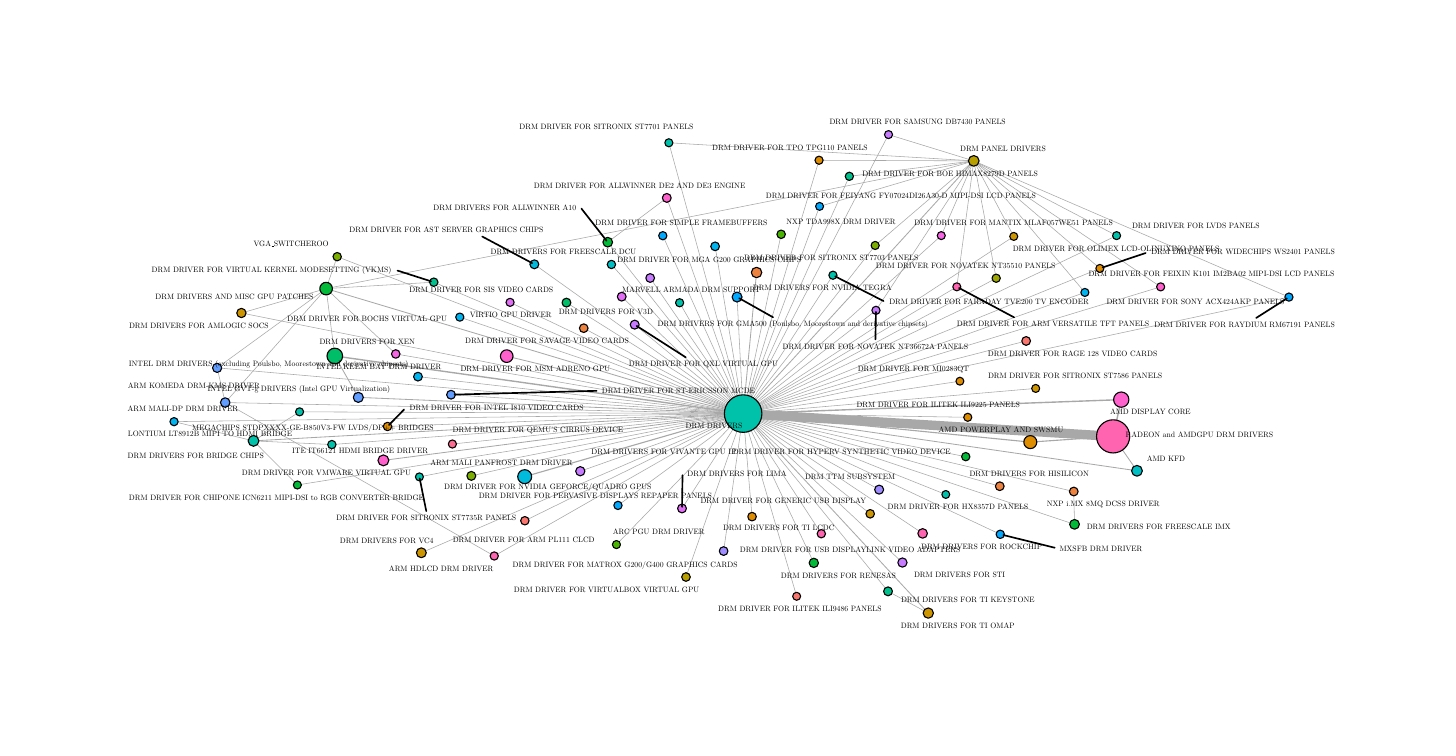
\begin{tikzpicture}[x=1pt,y=1pt]
\definecolor{fillColor}{RGB}{255,255,255}
\path[use as bounding box,fill=fillColor,fill opacity=0.00] (0,0) rectangle (505.89,252.94);
\begin{scope}
\path[clip] (  0.00,  0.00) rectangle (505.89,252.94);
\definecolor{fillColor}{RGB}{255,255,255}

\path[fill=fillColor] (  0.00,  0.00) rectangle (505.89,252.94);
\end{scope}
\begin{scope}
\path[clip] ( 32.75, 32.75) rectangle (475.89,222.94);
\definecolor{drawColor}{gray}{0.66}

\path[draw=drawColor,line width= 0.5pt,line join=round] (395.16,118.53) -- (258.53,113.49);

\path[draw=drawColor,line width= 0.5pt,line join=round] (395.16,118.53) -- (392.22,105.25);

\path[draw=drawColor,line width= 0.3pt,line join=round] (400.84, 92.82) -- (258.53,113.49);

\path[draw=drawColor,line width= 0.3pt,line join=round] (400.84, 92.82) -- (392.22,105.25);

\path[draw=drawColor,line width= 0.4pt,line join=round] (362.30,103.18) -- (258.53,113.49);

\path[draw=drawColor,line width= 0.4pt,line join=round] (362.30,103.18) -- (392.22,105.25);

\path[draw=drawColor,line width= 0.2pt,line join=round] (212.75, 66.16) -- (258.53,113.49);

\path[draw=drawColor,line width= 0.2pt,line join=round] (168.59, 62.04) -- ( 71.38,117.48);

\path[draw=drawColor,line width= 0.2pt,line join=round] (168.59, 62.04) -- (258.53,113.49);

\path[draw=drawColor,line width= 0.2pt,line join=round] ( 68.46,130.01) -- ( 71.38,117.48);

\path[draw=drawColor,line width= 0.2pt,line join=round] ( 68.46,130.01) -- (258.53,113.49);

\path[draw=drawColor,line width= 0.2pt,line join=round] ( 68.46,130.01) -- (107.84,158.65);

\path[draw=drawColor,line width= 0.2pt,line join=round] (160.31, 90.98) -- (258.53,113.49);

\path[draw=drawColor,line width= 0.2pt,line join=round] ( 71.38,117.48) -- (258.53,113.49);

\path[draw=drawColor,line width= 0.2pt,line join=round] ( 71.38,117.48) -- (107.84,158.65);

\path[draw=drawColor,line width= 0.2pt,line join=round] (230.94,191.42) -- (258.53,113.49);

\path[draw=drawColor,line width= 0.2pt,line join=round] (230.94,191.42) -- (209.60,175.43);

\path[draw=drawColor,line width= 0.2pt,line join=round] (179.65, 74.77) -- (258.53,113.49);

\path[draw=drawColor,line width= 0.2pt,line join=round] (335.74,159.30) -- (258.53,113.49);

\path[draw=drawColor,line width= 0.2pt,line join=round] (335.74,159.30) -- (341.87,204.80);

\path[draw=drawColor,line width= 0.2pt,line join=round] (183.09,167.43) -- (258.53,113.49);

\path[draw=drawColor,line width= 0.2pt,line join=round] (156.15,148.35) -- (258.53,113.49);

\path[draw=drawColor,line width= 0.2pt,line join=round] (296.91,199.23) -- (258.53,113.49);

\path[draw=drawColor,line width= 0.2pt,line join=round] (296.91,199.23) -- (341.87,204.80);

\path[draw=drawColor,line width= 0.2pt,line join=round] ( 97.45, 87.69) -- (258.53,113.49);

\path[draw=drawColor,line width= 0.2pt,line join=round] ( 97.45, 87.69) -- ( 81.61,103.63);

\path[draw=drawColor,line width= 0.2pt,line join=round] (290.98,163.49) -- (258.53,113.49);

\path[draw=drawColor,line width= 0.2pt,line join=round] (409.40,159.28) -- (258.53,113.49);

\path[draw=drawColor,line width= 0.2pt,line join=round] (409.40,159.28) -- (341.87,204.80);

\path[draw=drawColor,line width= 0.2pt,line join=round] (286.15,188.36) -- (258.53,113.49);

\path[draw=drawColor,line width= 0.2pt,line join=round] (286.15,188.36) -- (341.87,204.80);

\path[draw=drawColor,line width= 0.2pt,line join=round] (304.44, 77.28) -- (258.53,113.49);

\path[draw=drawColor,line width= 0.2pt,line join=round] (235.58,153.54) -- (258.53,113.49);

\path[draw=drawColor,line width= 0.2pt,line join=round] (331.76, 84.26) -- (258.53,113.49);

\path[draw=drawColor,line width= 0.2pt,line join=round] (338.97, 97.93) -- (258.53,113.49);

\path[draw=drawColor,line width= 0.2pt,line join=round] (339.70,112.15) -- (258.53,113.49);

\path[draw=drawColor,line width= 0.2pt,line join=round] (277.87, 47.47) -- (258.53,113.49);

\path[draw=drawColor,line width= 0.2pt,line join=round] (130.03,108.83) -- (258.53,113.49);

\path[draw=drawColor,line width= 0.2pt,line join=round] (393.48,177.79) -- (258.53,113.49);

\path[draw=drawColor,line width= 0.2pt,line join=round] (393.48,177.79) -- (341.87,204.80);

\path[draw=drawColor,line width= 0.2pt,line join=round] (330.12,177.80) -- (258.53,113.49);

\path[draw=drawColor,line width= 0.2pt,line join=round] (330.12,177.80) -- (341.87,204.80);

\path[draw=drawColor,line width= 0.2pt,line join=round] (251.48, 63.81) -- (258.53,113.49);

\path[draw=drawColor,line width= 0.2pt,line join=round] (248.40,173.92) -- (258.53,113.49);

\path[draw=drawColor,line width= 0.2pt,line join=round] (336.86,125.19) -- (258.53,113.49);

\path[draw=drawColor,line width= 0.3pt,line join=round] (173.10,134.25) -- (258.53,113.49);

\path[draw=drawColor,line width= 0.2pt,line join=round] (349.96,162.40) -- (258.53,113.49);

\path[draw=drawColor,line width= 0.2pt,line join=round] (349.96,162.40) -- (341.87,204.80);

\path[draw=drawColor,line width= 0.2pt,line join=round] (306.53,150.79) -- (258.53,113.49);

\path[draw=drawColor,line width= 0.2pt,line join=round] (306.53,150.79) -- (341.87,204.80);

\path[draw=drawColor,line width= 0.4pt,line join=round] (179.60, 90.70) -- (258.53,113.49);

\path[draw=drawColor,line width= 0.2pt,line join=round] (356.32,177.51) -- (258.53,113.49);

\path[draw=drawColor,line width= 0.2pt,line join=round] (356.32,177.51) -- (341.87,204.80);

\path[draw=drawColor,line width= 0.2pt,line join=round] (213.30, 80.31) -- (258.53,113.49);

\path[draw=drawColor,line width= 0.2pt,line join=round] (153.47,102.49) -- (258.53,113.49);

\path[draw=drawColor,line width= 0.2pt,line join=round] (219.34,145.63) -- (258.53,113.49);

\path[draw=drawColor,line width= 0.2pt,line join=round] (360.79,139.73) -- (258.53,113.49);

\path[draw=drawColor,line width= 0.2pt,line join=round] (455.75,155.58) -- (258.53,113.49);

\path[draw=drawColor,line width= 0.2pt,line join=round] (455.75,155.58) -- (341.87,204.80);

\path[draw=drawColor,line width= 0.2pt,line join=round] (311.06,214.30) -- (258.53,113.49);

\path[draw=drawColor,line width= 0.2pt,line join=round] (311.06,214.30) -- (341.87,204.80);

\path[draw=drawColor,line width= 0.2pt,line join=round] (200.93,144.35) -- (258.53,113.49);

\path[draw=drawColor,line width= 0.2pt,line join=round] (229.50,177.76) -- (258.53,113.49);

\path[draw=drawColor,line width= 0.2pt,line join=round] (174.31,153.68) -- (258.53,113.49);

\path[draw=drawColor,line width= 0.2pt,line join=round] (364.25,122.58) -- (258.53,113.49);

\path[draw=drawColor,line width= 0.2pt,line join=round] (231.68,211.35) -- (258.53,113.49);

\path[draw=drawColor,line width= 0.2pt,line join=round] (231.68,211.35) -- (341.87,204.80);

\path[draw=drawColor,line width= 0.2pt,line join=round] (306.24,174.24) -- (258.53,113.49);

\path[draw=drawColor,line width= 0.2pt,line join=round] (306.24,174.24) -- (341.87,204.80);

\path[draw=drawColor,line width= 0.2pt,line join=round] (141.55, 90.62) -- (258.53,113.49);

\path[draw=drawColor,line width= 0.2pt,line join=round] (382.02,157.26) -- (258.53,113.49);

\path[draw=drawColor,line width= 0.2pt,line join=round] (382.02,157.26) -- (341.87,204.80);

\path[draw=drawColor,line width= 0.2pt,line join=round] (152.97,120.31) -- (258.53,113.49);

\path[draw=drawColor,line width= 0.2pt,line join=round] (285.96,205.03) -- (258.53,113.49);

\path[draw=drawColor,line width= 0.2pt,line join=round] (285.96,205.03) -- (341.87,204.80);

\path[draw=drawColor,line width= 0.2pt,line join=round] (286.78, 70.08) -- (258.53,113.49);

\path[draw=drawColor,line width= 0.2pt,line join=round] (146.75,160.97) -- (258.53,113.49);

\path[draw=drawColor,line width= 0.2pt,line join=round] (146.75,160.97) -- (107.84,158.65);

\path[draw=drawColor,line width= 0.2pt,line join=round] (237.88, 54.43) -- (258.53,113.49);

\path[draw=drawColor,line width= 0.3pt,line join=round] (128.54, 96.58) -- (258.53,113.49);

\path[draw=drawColor,line width= 0.2pt,line join=round] (387.44,165.94) -- (258.53,113.49);

\path[draw=drawColor,line width= 0.2pt,line join=round] (387.44,165.94) -- (341.87,204.80);

\path[draw=drawColor,line width= 0.3pt,line join=round] (258.53,113.49) -- (107.84,158.65);

\path[draw=drawColor,line width= 0.2pt,line join=round] (258.53,113.49) -- (209.60,175.43);

\path[draw=drawColor,line width= 0.2pt,line join=round] (258.53,113.49) -- ( 77.23,149.84);

\path[draw=drawColor,line width= 0.3pt,line join=round] (258.53,113.49) -- ( 81.61,103.63);

\path[draw=drawColor,line width= 0.2pt,line join=round] (258.53,113.49) -- (210.93,167.37);

\path[draw=drawColor,line width= 0.2pt,line join=round] (258.53,113.49) -- (378.28, 73.47);

\path[draw=drawColor,line width= 0.2pt,line join=round] (258.53,113.49) -- (256.33,155.60);

\path[draw=drawColor,line width= 0.2pt,line join=round] (258.53,113.49) -- (351.26, 87.24);

\path[draw=drawColor,line width= 0.2pt,line join=round] (258.53,113.49) -- (236.44, 79.21);

\path[draw=drawColor,line width= 0.3pt,line join=round] (258.53,113.49) -- (263.38,164.47);

\path[draw=drawColor,line width= 0.2pt,line join=round] (258.53,113.49) -- (284.07, 59.54);

\path[draw=drawColor,line width= 0.2pt,line join=round] (258.53,113.49) -- (323.39, 70.19);

\path[draw=drawColor,line width= 0.2pt,line join=round] (258.53,113.49) -- (316.09, 59.66);

\path[draw=drawColor,line width= 0.2pt,line join=round] (258.53,113.49) -- (310.89, 49.26);

\path[draw=drawColor,line width= 0.2pt,line join=round] (258.53,113.49) -- (261.75, 76.25);

\path[draw=drawColor,line width= 0.3pt,line join=round] (258.53,113.49) -- (325.43, 41.40);

\path[draw=drawColor,line width= 0.2pt,line join=round] (258.53,113.49) -- (214.66,155.74);

\path[draw=drawColor,line width= 0.2pt,line join=round] (258.53,113.49) -- (142.25, 63.19);

\path[draw=drawColor,line width= 0.2pt,line join=round] (258.53,113.49) -- (199.69, 92.66);

\path[draw=drawColor,line width= 0.2pt,line join=round] (258.53,113.49) -- (133.00,135.03);

\path[draw=drawColor,line width= 0.3pt,line join=round] (258.53,113.49) -- (341.87,204.80);

\path[draw=drawColor,line width= 0.2pt,line join=round] (258.53,113.49) -- (307.68, 86.01);

\path[draw=drawColor,line width= 0.5pt,line join=round] (258.53,113.49) -- (110.98,134.30);

\path[draw=drawColor,line width= 0.3pt,line join=round] (258.53,113.49) -- (119.47,119.35);

\path[draw=drawColor,line width= 0.2pt,line join=round] (258.53,113.49) -- (141.03,126.84);

\path[draw=drawColor,line width= 0.2pt,line join=round] (258.53,113.49) -- (109.91,102.30);

\path[draw=drawColor,line width= 0.2pt,line join=round] (258.53,113.49) -- ( 52.89,110.57);

\path[draw=drawColor,line width= 0.2pt,line join=round] (258.53,113.49) -- (224.94,162.48);

\path[draw=drawColor,line width= 0.2pt,line join=round] (258.53,113.49) -- ( 98.25,114.12);

\path[draw=drawColor,line width= 0.2pt,line join=round] (258.53,113.49) -- (351.44, 69.87);

\path[draw=drawColor,line width= 0.2pt,line join=round] (258.53,113.49) -- (272.26,178.28);

\path[draw=drawColor,line width= 0.2pt,line join=round] (258.53,113.49) -- (378.00, 85.33);

\path[draw=drawColor,line width= 3.4pt,line join=round] (258.53,113.49) -- (392.22,105.25);

\path[draw=drawColor,line width= 0.2pt,line join=round] (258.53,113.49) -- (111.84,170.19);

\path[draw=drawColor,line width= 0.2pt,line join=round] (258.53,113.49) -- (194.69,153.59);

\path[draw=drawColor,line width= 0.2pt,line join=round] (107.84,158.65) -- ( 77.23,149.84);

\path[draw=drawColor,line width= 0.2pt,line join=round] (107.84,158.65) -- (133.00,135.03);

\path[draw=drawColor,line width= 0.2pt,line join=round] (107.84,158.65) -- (341.87,204.80);

\path[draw=drawColor,line width= 0.2pt,line join=round] (107.84,158.65) -- (110.98,134.30);

\path[draw=drawColor,line width= 0.2pt,line join=round] (107.84,158.65) -- (111.84,170.19);

\path[draw=drawColor,line width= 0.2pt,line join=round] ( 81.61,103.63) -- (109.91,102.30);

\path[draw=drawColor,line width= 0.2pt,line join=round] ( 81.61,103.63) -- ( 52.89,110.57);

\path[draw=drawColor,line width= 0.2pt,line join=round] ( 81.61,103.63) -- ( 98.25,114.12);

\path[draw=drawColor,line width= 0.2pt,line join=round] (378.28, 73.47) -- (378.00, 85.33);

\path[draw=drawColor,line width= 0.2pt,line join=round] (310.89, 49.26) -- (325.43, 41.40);

\path[draw=drawColor,line width= 0.3pt,line join=round] (110.98,134.30) -- (119.47,119.35);
\definecolor{drawColor}{RGB}{0,0,0}
\definecolor{fillColor}{RGB}{255,97,204}

\path[draw=drawColor,line width= 0.4pt,line join=round,line cap=round,fill=fillColor] (395.16,118.53) circle (  2.76);
\definecolor{fillColor}{RGB}{0,191,196}

\path[draw=drawColor,line width= 0.4pt,line join=round,line cap=round,fill=fillColor] (400.84, 92.82) circle (  1.95);
\definecolor{fillColor}{RGB}{222,140,0}

\path[draw=drawColor,line width= 0.4pt,line join=round,line cap=round,fill=fillColor] (362.30,103.18) circle (  2.35);
\definecolor{fillColor}{RGB}{73,181,0}

\path[draw=drawColor,line width= 0.4pt,line join=round,line cap=round,fill=fillColor] (212.75, 66.16) circle (  1.46);
\definecolor{fillColor}{RGB}{255,100,176}

\path[draw=drawColor,line width= 0.4pt,line join=round,line cap=round,fill=fillColor] (168.59, 62.04) circle (  1.49);
\definecolor{fillColor}{RGB}{97,156,255}

\path[draw=drawColor,line width= 0.4pt,line join=round,line cap=round,fill=fillColor] ( 68.46,130.01) circle (  1.66);
\definecolor{fillColor}{RGB}{124,174,0}

\path[draw=drawColor,line width= 0.4pt,line join=round,line cap=round,fill=fillColor] (160.31, 90.98) circle (  1.61);
\definecolor{fillColor}{RGB}{97,156,255}

\path[draw=drawColor,line width= 0.4pt,line join=round,line cap=round,fill=fillColor] ( 71.38,117.48) circle (  1.72);
\definecolor{fillColor}{RGB}{255,97,204}

\path[draw=drawColor,line width= 0.4pt,line join=round,line cap=round,fill=fillColor] (230.94,191.42) circle (  1.60);
\definecolor{fillColor}{RGB}{248,118,109}

\path[draw=drawColor,line width= 0.4pt,line join=round,line cap=round,fill=fillColor] (179.65, 74.77) circle (  1.52);
\definecolor{fillColor}{RGB}{255,100,176}

\path[draw=drawColor,line width= 0.4pt,line join=round,line cap=round,fill=fillColor] (335.74,159.30) circle (  1.45);
\definecolor{fillColor}{RGB}{0,187,220}

\path[draw=drawColor,line width= 0.4pt,line join=round,line cap=round,fill=fillColor] (183.09,167.43) circle (  1.61);
\definecolor{fillColor}{RGB}{0,180,240}

\path[draw=drawColor,line width= 0.4pt,line join=round,line cap=round,fill=fillColor] (156.15,148.35) circle (  1.48);
\definecolor{fillColor}{RGB}{0,192,139}

\path[draw=drawColor,line width= 0.4pt,line join=round,line cap=round,fill=fillColor] (296.91,199.23) circle (  1.49);
\definecolor{fillColor}{RGB}{0,186,56}

\path[draw=drawColor,line width= 0.4pt,line join=round,line cap=round,fill=fillColor] ( 97.45, 87.69) circle (  1.45);
\definecolor{fillColor}{RGB}{0,193,169}

\path[draw=drawColor,line width= 0.4pt,line join=round,line cap=round,fill=fillColor] (290.98,163.49) circle (  1.48);
\definecolor{fillColor}{RGB}{255,97,204}

\path[draw=drawColor,line width= 0.4pt,line join=round,line cap=round,fill=fillColor] (409.40,159.28) circle (  1.47);
\definecolor{fillColor}{RGB}{0,169,255}

\path[draw=drawColor,line width= 0.4pt,line join=round,line cap=round,fill=fillColor] (286.15,188.36) circle (  1.43);
\definecolor{fillColor}{RGB}{205,150,0}

\path[draw=drawColor,line width= 0.4pt,line join=round,line cap=round,fill=fillColor] (304.44, 77.28) circle (  1.54);
\definecolor{fillColor}{RGB}{0,193,169}

\path[draw=drawColor,line width= 0.4pt,line join=round,line cap=round,fill=fillColor] (235.58,153.54) circle (  1.48);

\path[draw=drawColor,line width= 0.4pt,line join=round,line cap=round,fill=fillColor] (331.76, 84.26) circle (  1.43);
\definecolor{fillColor}{RGB}{0,186,56}

\path[draw=drawColor,line width= 0.4pt,line join=round,line cap=round,fill=fillColor] (338.97, 97.93) circle (  1.50);
\definecolor{fillColor}{RGB}{222,140,0}

\path[draw=drawColor,line width= 0.4pt,line join=round,line cap=round,fill=fillColor] (339.70,112.15) circle (  1.46);
\definecolor{fillColor}{RGB}{248,118,109}

\path[draw=drawColor,line width= 0.4pt,line join=round,line cap=round,fill=fillColor] (277.87, 47.47) circle (  1.44);
\definecolor{fillColor}{RGB}{222,140,0}

\path[draw=drawColor,line width= 0.4pt,line join=round,line cap=round,fill=fillColor] (130.03,108.83) circle (  1.52);
\definecolor{fillColor}{RGB}{0,193,169}

\path[draw=drawColor,line width= 0.4pt,line join=round,line cap=round,fill=fillColor] (393.48,177.79) circle (  1.45);
\definecolor{fillColor}{RGB}{245,100,227}

\path[draw=drawColor,line width= 0.4pt,line join=round,line cap=round,fill=fillColor] (330.12,177.80) circle (  1.45);
\definecolor{fillColor}{RGB}{159,140,255}

\path[draw=drawColor,line width= 0.4pt,line join=round,line cap=round,fill=fillColor] (251.48, 63.81) circle (  1.57);
\definecolor{fillColor}{RGB}{0,180,240}

\path[draw=drawColor,line width= 0.4pt,line join=round,line cap=round,fill=fillColor] (248.40,173.92) circle (  1.57);
\definecolor{fillColor}{RGB}{222,140,0}

\path[draw=drawColor,line width= 0.4pt,line join=round,line cap=round,fill=fillColor] (336.86,125.19) circle (  1.43);
\definecolor{fillColor}{RGB}{255,97,204}

\path[draw=drawColor,line width= 0.4pt,line join=round,line cap=round,fill=fillColor] (173.10,134.25) circle (  2.28);
\definecolor{fillColor}{RGB}{157,167,0}

\path[draw=drawColor,line width= 0.4pt,line join=round,line cap=round,fill=fillColor] (349.96,162.40) circle (  1.50);
\definecolor{fillColor}{RGB}{199,124,255}

\path[draw=drawColor,line width= 0.4pt,line join=round,line cap=round,fill=fillColor] (306.53,150.79) circle (  1.48);
\definecolor{fillColor}{RGB}{0,187,220}

\path[draw=drawColor,line width= 0.4pt,line join=round,line cap=round,fill=fillColor] (179.60, 90.70) circle (  2.52);
\definecolor{fillColor}{RGB}{205,150,0}

\path[draw=drawColor,line width= 0.4pt,line join=round,line cap=round,fill=fillColor] (356.32,177.51) circle (  1.45);
\definecolor{fillColor}{RGB}{0,169,255}

\path[draw=drawColor,line width= 0.4pt,line join=round,line cap=round,fill=fillColor] (213.30, 80.31) circle (  1.50);
\definecolor{fillColor}{RGB}{255,108,145}

\path[draw=drawColor,line width= 0.4pt,line join=round,line cap=round,fill=fillColor] (153.47,102.49) circle (  1.47);
\definecolor{fillColor}{RGB}{199,124,255}

\path[draw=drawColor,line width= 0.4pt,line join=round,line cap=round,fill=fillColor] (219.34,145.63) circle (  1.62);
\definecolor{fillColor}{RGB}{248,118,109}

\path[draw=drawColor,line width= 0.4pt,line join=round,line cap=round,fill=fillColor] (360.79,139.73) circle (  1.58);
\definecolor{fillColor}{RGB}{0,169,255}

\path[draw=drawColor,line width= 0.4pt,line join=round,line cap=round,fill=fillColor] (455.75,155.58) circle (  1.48);
\definecolor{fillColor}{RGB}{199,124,255}

\path[draw=drawColor,line width= 0.4pt,line join=round,line cap=round,fill=fillColor] (311.06,214.30) circle (  1.45);
\definecolor{fillColor}{RGB}{237,129,62}

\path[draw=drawColor,line width= 0.4pt,line join=round,line cap=round,fill=fillColor] (200.93,144.35) circle (  1.56);
\definecolor{fillColor}{RGB}{0,169,255}

\path[draw=drawColor,line width= 0.4pt,line join=round,line cap=round,fill=fillColor] (229.50,177.76) circle (  1.49);
\definecolor{fillColor}{RGB}{227,110,246}

\path[draw=drawColor,line width= 0.4pt,line join=round,line cap=round,fill=fillColor] (174.31,153.68) circle (  1.47);
\definecolor{fillColor}{RGB}{205,150,0}

\path[draw=drawColor,line width= 0.4pt,line join=round,line cap=round,fill=fillColor] (364.25,122.58) circle (  1.45);
\definecolor{fillColor}{RGB}{0,193,169}

\path[draw=drawColor,line width= 0.4pt,line join=round,line cap=round,fill=fillColor] (231.68,211.35) circle (  1.46);
\definecolor{fillColor}{RGB}{124,174,0}

\path[draw=drawColor,line width= 0.4pt,line join=round,line cap=round,fill=fillColor] (306.24,174.24) circle (  1.47);
\definecolor{fillColor}{RGB}{0,193,169}

\path[draw=drawColor,line width= 0.4pt,line join=round,line cap=round,fill=fillColor] (141.55, 90.62) circle (  1.44);
\definecolor{fillColor}{RGB}{0,180,240}

\path[draw=drawColor,line width= 0.4pt,line join=round,line cap=round,fill=fillColor] (382.02,157.26) circle (  1.46);
\definecolor{fillColor}{RGB}{97,156,255}

\path[draw=drawColor,line width= 0.4pt,line join=round,line cap=round,fill=fillColor] (152.97,120.31) circle (  1.59);
\definecolor{fillColor}{RGB}{222,140,0}

\path[draw=drawColor,line width= 0.4pt,line join=round,line cap=round,fill=fillColor] (285.96,205.03) circle (  1.47);
\definecolor{fillColor}{RGB}{255,100,176}

\path[draw=drawColor,line width= 0.4pt,line join=round,line cap=round,fill=fillColor] (286.78, 70.08) circle (  1.51);
\definecolor{fillColor}{RGB}{0,192,139}

\path[draw=drawColor,line width= 0.4pt,line join=round,line cap=round,fill=fillColor] (146.75,160.97) circle (  1.52);
\definecolor{fillColor}{RGB}{183,159,0}

\path[draw=drawColor,line width= 0.4pt,line join=round,line cap=round,fill=fillColor] (237.88, 54.43) circle (  1.55);
\definecolor{fillColor}{RGB}{255,97,204}

\path[draw=drawColor,line width= 0.4pt,line join=round,line cap=round,fill=fillColor] (128.54, 96.58) circle (  1.97);
\definecolor{fillColor}{RGB}{222,140,0}

\path[draw=drawColor,line width= 0.4pt,line join=round,line cap=round,fill=fillColor] (387.44,165.94) circle (  1.46);
\definecolor{fillColor}{RGB}{0,193,169}

\path[draw=drawColor,line width= 0.4pt,line join=round,line cap=round,fill=fillColor] (258.53,113.49) circle (  6.78);
\definecolor{fillColor}{RGB}{0,186,56}

\path[draw=drawColor,line width= 0.4pt,line join=round,line cap=round,fill=fillColor] (107.84,158.65) circle (  2.27);

\path[draw=drawColor,line width= 0.4pt,line join=round,line cap=round,fill=fillColor] (209.60,175.43) circle (  1.75);
\definecolor{fillColor}{RGB}{205,150,0}

\path[draw=drawColor,line width= 0.4pt,line join=round,line cap=round,fill=fillColor] ( 77.23,149.84) circle (  1.68);
\definecolor{fillColor}{RGB}{0,193,169}

\path[draw=drawColor,line width= 0.4pt,line join=round,line cap=round,fill=fillColor] ( 81.61,103.63) circle (  1.95);
\definecolor{fillColor}{RGB}{0,191,196}

\path[draw=drawColor,line width= 0.4pt,line join=round,line cap=round,fill=fillColor] (210.93,167.37) circle (  1.51);
\definecolor{fillColor}{RGB}{0,186,56}

\path[draw=drawColor,line width= 0.4pt,line join=round,line cap=round,fill=fillColor] (378.28, 73.47) circle (  1.76);
\definecolor{fillColor}{RGB}{0,169,255}

\path[draw=drawColor,line width= 0.4pt,line join=round,line cap=round,fill=fillColor] (256.33,155.60) circle (  1.80);
\definecolor{fillColor}{RGB}{237,129,62}

\path[draw=drawColor,line width= 0.4pt,line join=round,line cap=round,fill=fillColor] (351.26, 87.24) circle (  1.58);
\definecolor{fillColor}{RGB}{227,110,246}

\path[draw=drawColor,line width= 0.4pt,line join=round,line cap=round,fill=fillColor] (236.44, 79.21) circle (  1.60);
\definecolor{fillColor}{RGB}{237,129,62}

\path[draw=drawColor,line width= 0.4pt,line join=round,line cap=round,fill=fillColor] (263.38,164.47) circle (  1.89);
\definecolor{fillColor}{RGB}{0,186,56}

\path[draw=drawColor,line width= 0.4pt,line join=round,line cap=round,fill=fillColor] (284.07, 59.54) circle (  1.68);
\definecolor{fillColor}{RGB}{255,100,176}

\path[draw=drawColor,line width= 0.4pt,line join=round,line cap=round,fill=fillColor] (323.39, 70.19) circle (  1.73);
\definecolor{fillColor}{RGB}{199,124,255}

\path[draw=drawColor,line width= 0.4pt,line join=round,line cap=round,fill=fillColor] (316.09, 59.66) circle (  1.67);
\definecolor{fillColor}{RGB}{0,192,139}

\path[draw=drawColor,line width= 0.4pt,line join=round,line cap=round,fill=fillColor] (310.89, 49.26) circle (  1.60);
\definecolor{fillColor}{RGB}{222,140,0}

\path[draw=drawColor,line width= 0.4pt,line join=round,line cap=round,fill=fillColor] (261.75, 76.25) circle (  1.55);
\definecolor{fillColor}{RGB}{205,150,0}

\path[draw=drawColor,line width= 0.4pt,line join=round,line cap=round,fill=fillColor] (325.43, 41.40) circle (  1.86);
\definecolor{fillColor}{RGB}{227,110,246}

\path[draw=drawColor,line width= 0.4pt,line join=round,line cap=round,fill=fillColor] (214.66,155.74) circle (  1.59);
\definecolor{fillColor}{RGB}{205,150,0}

\path[draw=drawColor,line width= 0.4pt,line join=round,line cap=round,fill=fillColor] (142.25, 63.19) circle (  1.78);
\definecolor{fillColor}{RGB}{199,124,255}

\path[draw=drawColor,line width= 0.4pt,line join=round,line cap=round,fill=fillColor] (199.69, 92.66) circle (  1.67);
\definecolor{fillColor}{RGB}{245,100,227}

\path[draw=drawColor,line width= 0.4pt,line join=round,line cap=round,fill=fillColor] (133.00,135.03) circle (  1.54);
\definecolor{fillColor}{RGB}{183,159,0}

\path[draw=drawColor,line width= 0.4pt,line join=round,line cap=round,fill=fillColor] (341.87,204.80) circle (  1.93);
\definecolor{fillColor}{RGB}{159,140,255}

\path[draw=drawColor,line width= 0.4pt,line join=round,line cap=round,fill=fillColor] (307.68, 86.01) circle (  1.63);
\definecolor{fillColor}{RGB}{0,190,103}

\path[draw=drawColor,line width= 0.4pt,line join=round,line cap=round,fill=fillColor] (110.98,134.30) circle (  2.82);
\definecolor{fillColor}{RGB}{97,156,255}

\path[draw=drawColor,line width= 0.4pt,line join=round,line cap=round,fill=fillColor] (119.47,119.35) circle (  1.82);
\definecolor{fillColor}{RGB}{0,180,240}

\path[draw=drawColor,line width= 0.4pt,line join=round,line cap=round,fill=fillColor] (141.03,126.84) circle (  1.58);
\definecolor{fillColor}{RGB}{0,193,169}

\path[draw=drawColor,line width= 0.4pt,line join=round,line cap=round,fill=fillColor] (109.91,102.30) circle (  1.50);
\definecolor{fillColor}{RGB}{0,180,240}

\path[draw=drawColor,line width= 0.4pt,line join=round,line cap=round,fill=fillColor] ( 52.89,110.57) circle (  1.48);
\definecolor{fillColor}{RGB}{199,124,255}

\path[draw=drawColor,line width= 0.4pt,line join=round,line cap=round,fill=fillColor] (224.94,162.48) circle (  1.58);
\definecolor{fillColor}{RGB}{0,193,169}

\path[draw=drawColor,line width= 0.4pt,line join=round,line cap=round,fill=fillColor] ( 98.25,114.12) circle (  1.46);
\definecolor{fillColor}{RGB}{0,169,255}

\path[draw=drawColor,line width= 0.4pt,line join=round,line cap=round,fill=fillColor] (351.44, 69.87) circle (  1.51);
\definecolor{fillColor}{RGB}{73,181,0}

\path[draw=drawColor,line width= 0.4pt,line join=round,line cap=round,fill=fillColor] (272.26,178.28) circle (  1.53);
\definecolor{fillColor}{RGB}{237,129,62}

\path[draw=drawColor,line width= 0.4pt,line join=round,line cap=round,fill=fillColor] (378.00, 85.33) circle (  1.58);
\definecolor{fillColor}{RGB}{255,100,176}

\path[draw=drawColor,line width= 0.4pt,line join=round,line cap=round,fill=fillColor] (392.22,105.25) circle (  5.99);
\definecolor{fillColor}{RGB}{124,174,0}

\path[draw=drawColor,line width= 0.4pt,line join=round,line cap=round,fill=fillColor] (111.84,170.19) circle (  1.51);
\definecolor{fillColor}{RGB}{0,190,103}

\path[draw=drawColor,line width= 0.4pt,line join=round,line cap=round,fill=fillColor] (194.69,153.59) circle (  1.60);

\path[draw=drawColor,line width= 0.6pt,line join=round,line cap=round] (356.45,148.25) -- (336.54,158.88);

\path[draw=drawColor,line width= 0.6pt,line join=round,line cap=round] (164.25,177.47) -- (182.29,167.86);

\path[draw=drawColor,line width= 0.6pt,line join=round,line cap=round] (309.26,154.15) -- (291.80,163.07);

\path[draw=drawColor,line width= 0.6pt,line join=round,line cap=round] (136.03,114.97) -- (130.52,109.34);

\path[draw=drawColor,line width= 0.6pt,line join=round,line cap=round] (306.33,140.29) -- (306.52,150.24);

\path[draw=drawColor,line width= 0.6pt,line join=round,line cap=round] (237.79,133.82) -- (220.05,145.18);

\path[draw=drawColor,line width= 0.6pt,line join=round,line cap=round] (443.92,148.05) -- (455.04,155.12);

\path[draw=drawColor,line width= 0.6pt,line join=round,line cap=round] (144.03, 78.26) -- (141.66, 90.07);

\path[draw=drawColor,line width= 0.6pt,line join=round,line cap=round] (205.58,121.71) -- (154.24,120.35);

\path[draw=drawColor,line width= 0.6pt,line join=round,line cap=round] (133.63,165.17) -- (145.74,161.29);

\path[draw=drawColor,line width= 0.6pt,line join=round,line cap=round] (403.98,171.52) -- (388.44,166.28);

\path[draw=drawColor,line width= 0.6pt,line join=round,line cap=round] (200.09,187.57) -- (209.19,175.94);

\path[draw=drawColor,line width= 0.6pt,line join=round,line cap=round] (269.35,148.28) -- (257.11,155.17);

\path[draw=drawColor,line width= 0.6pt,line join=round,line cap=round] (236.63, 91.25) -- (236.45, 79.76);

\path[draw=drawColor,line width= 0.6pt,line join=round,line cap=round] (371.12, 65.02) -- (352.54, 69.60);

\node[text=drawColor,anchor=base,inner sep=0pt, outer sep=0pt, scale=  0.28] at (405.70,113.03) {AMD DISPLAY CORE};

\node[text=drawColor,anchor=base,inner sep=0pt, outer sep=0pt, scale=  0.28] at (411.32, 96.35) {AMD KFD};

\node[text=drawColor,anchor=base,inner sep=0pt, outer sep=0pt, scale=  0.28] at (351.71,106.75) {AMD POWERPLAY AND SWSMU};

\node[text=drawColor,anchor=base,inner sep=0pt, outer sep=0pt, scale=  0.28] at (228.04, 69.74) {ARC PGU DRM DRIVER};

\node[text=drawColor,anchor=base,inner sep=0pt, outer sep=0pt, scale=  0.28] at (149.42, 56.51) {ARM HDLCD DRM DRIVER};

\node[text=drawColor,anchor=base,inner sep=0pt, outer sep=0pt, scale=  0.28] at ( 60.04,122.59) {ARM KOMEDA DRM-KMS DRIVER};

\node[text=drawColor,anchor=base,inner sep=0pt, outer sep=0pt, scale=  0.28] at (171.19, 94.58) {ARM MALI PANFROST DRM DRIVER};

\node[text=drawColor,anchor=base,inner sep=0pt, outer sep=0pt, scale=  0.28] at ( 56.07,114.16) {ARM MALI-DP DRM DRIVER};

\node[text=drawColor,anchor=base,inner sep=0pt, outer sep=0pt, scale=  0.28] at (221.14,194.98) {DRM DRIVER FOR ALLWINNER DE2 AND DE3 ENGINE};

\node[text=drawColor,anchor=base,inner sep=0pt, outer sep=0pt, scale=  0.28] at (179.22, 66.82) {DRM DRIVER FOR ARM PL111 CLCD};

\node[text=drawColor,anchor=base,inner sep=0pt, outer sep=0pt, scale=  0.28] at (370.54,144.78) {DRM DRIVER FOR ARM VERSATILE TFT PANELS};

\node[text=drawColor,anchor=base,inner sep=0pt, outer sep=0pt, scale=  0.28] at (151.32,178.98) {DRM DRIVER FOR AST SERVER GRAPHICS CHIPS};

\node[text=drawColor,anchor=base,inner sep=0pt, outer sep=0pt, scale=  0.28] at (122.68,146.83) {DRM DRIVER FOR BOCHS VIRTUAL GPU};

\node[text=drawColor,anchor=base,inner sep=0pt, outer sep=0pt, scale=  0.28] at (333.33,199.29) {DRM DRIVER FOR BOE HIMAX8279D PANELS};

\node[text=drawColor,anchor=base,inner sep=0pt, outer sep=0pt, scale=  0.28] at ( 89.90, 82.19) {DRM DRIVER FOR CHIPONE ICN6211 MIPI-DSI to RGB CONVERTER BRIDGE};

\node[text=drawColor,anchor=base,inner sep=0pt, outer sep=0pt, scale=  0.28] at (347.39,152.80) {DRM DRIVER FOR FARADAY TVE200 TV ENCODER};

\node[text=drawColor,anchor=base,inner sep=0pt, outer sep=0pt, scale=  0.28] at (427.76,162.85) {DRM DRIVER FOR FEIXIN K101 IM2BA02 MIPI-DSI LCD PANELS};

\node[text=drawColor,anchor=base,inner sep=0pt, outer sep=0pt, scale=  0.28] at (315.56,191.31) {DRM DRIVER FOR FEIYANG FY07024DI26A30-D MIPI-DSI LCD PANELS};

\node[text=drawColor,anchor=base,inner sep=0pt, outer sep=0pt, scale=  0.28] at (273.07, 80.84) {DRM DRIVER FOR GENERIC USB DISPLAY};

\node[text=drawColor,anchor=base,inner sep=0pt, outer sep=0pt, scale=  0.28] at (336.16, 78.72) {DRM DRIVER FOR HX8357D PANELS};

\node[text=drawColor,anchor=base,inner sep=0pt, outer sep=0pt, scale=  0.28] at (294.16, 98.78) {DRM DRIVER FOR HYPERV SYNTHETIC VIDEO DEVICE};

\node[text=drawColor,anchor=base,inner sep=0pt, outer sep=0pt, scale=  0.28] at (329.03,115.70) {DRM DRIVER FOR ILITEK ILI9225 PANELS};

\node[text=drawColor,anchor=base,inner sep=0pt, outer sep=0pt, scale=  0.28] at (279.05, 41.89) {DRM DRIVER FOR ILITEK ILI9486 PANELS};

\node[text=drawColor,anchor=base,inner sep=0pt, outer sep=0pt, scale=  0.28] at (169.45,114.75) {DRM DRIVER FOR INTEL I810 VIDEO CARDS};

\node[text=drawColor,anchor=base,inner sep=0pt, outer sep=0pt, scale=  0.28] at (422.11,180.23) {DRM DRIVER FOR LVDS PANELS};

\node[text=drawColor,anchor=base,inner sep=0pt, outer sep=0pt, scale=  0.28] at (356.29,181.38) {DRM DRIVER FOR MANTIX MLAF057WE51 PANELS};

\node[text=drawColor,anchor=base,inner sep=0pt, outer sep=0pt, scale=  0.28] at (215.89, 57.99) {DRM DRIVER FOR MATROX G200/G400 GRAPHICS CARDS};

\node[text=drawColor,anchor=base,inner sep=0pt, outer sep=0pt, scale=  0.28] at (246.28,168.04) {DRM DRIVER FOR MGA G200 GRAPHICS CHIPS};

\node[text=drawColor,anchor=base,inner sep=0pt, outer sep=0pt, scale=  0.28] at (320.07,128.74) {DRM DRIVER FOR MI0283QT};

\node[text=drawColor,anchor=base,inner sep=0pt, outer sep=0pt, scale=  0.28] at (183.44,128.72) {DRM DRIVER FOR MSM ADRENO GPU};

\node[text=drawColor,anchor=base,inner sep=0pt, outer sep=0pt, scale=  0.28] at (338.97,166.00) {DRM DRIVER FOR NOVATEK NT35510 PANELS};

\node[text=drawColor,anchor=base,inner sep=0pt, outer sep=0pt, scale=  0.28] at (306.33,136.82) {DRM DRIVER FOR NOVATEK NT36672A PANELS};

\node[text=drawColor,anchor=base,inner sep=0pt, outer sep=0pt, scale=  0.28] at (187.94, 86.08) {DRM DRIVER FOR NVIDIA GEFORCE/QUADRO GPUS};

\node[text=drawColor,anchor=base,inner sep=0pt, outer sep=0pt, scale=  0.28] at (393.31,172.23) {DRM DRIVER FOR OLIMEX LCD-OLINUXINO PANELS};

\node[text=drawColor,anchor=base,inner sep=0pt, outer sep=0pt, scale=  0.28] at (205.13, 82.81) {DRM DRIVER FOR PERVASIVE DISPLAYS REPAPER PANELS};

\node[text=drawColor,anchor=base,inner sep=0pt, outer sep=0pt, scale=  0.28] at (184.37,106.74) {DRM DRIVER FOR QEMU'S CIRRUS DEVICE};

\node[text=drawColor,anchor=base,inner sep=0pt, outer sep=0pt, scale=  0.28] at (244.19,130.35) {DRM DRIVER FOR QXL VIRTUAL GPU};

\node[text=drawColor,anchor=base,inner sep=0pt, outer sep=0pt, scale=  0.28] at (377.60,134.21) {DRM DRIVER FOR RAGE 128 VIDEO CARDS};

\node[text=drawColor,anchor=base,inner sep=0pt, outer sep=0pt, scale=  0.28] at (439.73,144.58) {DRM DRIVER FOR RAYDIUM RM67191 PANELS};

\node[text=drawColor,anchor=base,inner sep=0pt, outer sep=0pt, scale=  0.28] at (321.59,217.83) {DRM DRIVER FOR SAMSUNG DB7430 PANELS};

\node[text=drawColor,anchor=base,inner sep=0pt, outer sep=0pt, scale=  0.28] at (187.69,138.84) {DRM DRIVER FOR SAVAGE VIDEO CARDS};

\node[text=drawColor,anchor=base,inner sep=0pt, outer sep=0pt, scale=  0.28] at (236.26,181.33) {DRM DRIVER FOR SIMPLE FRAMEBUFFERS};

\node[text=drawColor,anchor=base,inner sep=0pt, outer sep=0pt, scale=  0.28] at (163.91,157.22) {DRM DRIVER FOR SIS VIDEO CARDS};

\node[text=drawColor,anchor=base,inner sep=0pt, outer sep=0pt, scale=  0.28] at (378.49,126.19) {DRM DRIVER FOR SITRONIX ST7586 PANELS};

\node[text=drawColor,anchor=base,inner sep=0pt, outer sep=0pt, scale=  0.28] at (209.14,216.03) {DRM DRIVER FOR SITRONIX ST7701 PANELS};

\node[text=drawColor,anchor=base,inner sep=0pt, outer sep=0pt, scale=  0.28] at (290.37,168.73) {DRM DRIVER FOR SITRONIX ST7703 PANELS};

\node[text=drawColor,anchor=base,inner sep=0pt, outer sep=0pt, scale=  0.28] at (144.03, 74.80) {DRM DRIVER FOR SITRONIX ST7735R PANELS};

\node[text=drawColor,anchor=base,inner sep=0pt, outer sep=0pt, scale=  0.28] at (421.97,152.77) {DRM DRIVER FOR SONY ACX424AKP PANELS};

\node[text=drawColor,anchor=base,inner sep=0pt, outer sep=0pt, scale=  0.28] at (235.17,120.73) {DRM DRIVER FOR ST-ERICSSON MCDE};

\node[text=drawColor,anchor=base,inner sep=0pt, outer sep=0pt, scale=  0.28] at (275.47,208.61) {DRM DRIVER FOR TPO TPG110 PANELS};

\node[text=drawColor,anchor=base,inner sep=0pt, outer sep=0pt, scale=  0.28] at (297.18, 63.12) {DRM DRIVER FOR USB DISPLAYLINK VIDEO ADAPTERS};

\node[text=drawColor,anchor=base,inner sep=0pt, outer sep=0pt, scale=  0.28] at ( 88.13,164.62) {DRM DRIVER FOR VIRTUAL KERNEL MODESETTING (VKMS)};

\node[text=drawColor,anchor=base,inner sep=0pt, outer sep=0pt, scale=  0.28] at (209.16, 48.94) {DRM DRIVER FOR VIRTUALBOX VIRTUAL GPU};

\node[text=drawColor,anchor=base,inner sep=0pt, outer sep=0pt, scale=  0.28] at (107.98, 91.24) {DRM DRIVER FOR VMWARE VIRTUAL GPU};

\node[text=drawColor,anchor=base,inner sep=0pt, outer sep=0pt, scale=  0.28] at (439.18,170.91) {DRM DRIVER FOR WIDECHIPS WS2401 PANELS};

\node[text=drawColor,anchor=base,inner sep=0pt, outer sep=0pt, scale=  0.28] at (248.03,108.00) {DRM DRIVERS};

\node[text=drawColor,anchor=base,inner sep=0pt, outer sep=0pt, scale=  0.28] at ( 74.73,154.81) {DRM DRIVERS AND MISC GPU PATCHES};

\node[text=drawColor,anchor=base,inner sep=0pt, outer sep=0pt, scale=  0.28] at (172.40,187.02) {DRM DRIVERS FOR ALLWINNER A10};

\node[text=drawColor,anchor=base,inner sep=0pt, outer sep=0pt, scale=  0.28] at ( 61.86,144.33) {DRM DRIVERS FOR AMLOGIC SOCS};

\node[text=drawColor,anchor=base,inner sep=0pt, outer sep=0pt, scale=  0.28] at ( 60.76, 97.08) {DRM DRIVERS FOR BRIDGE CHIPS};

\node[text=drawColor,anchor=base,inner sep=0pt, outer sep=0pt, scale=  0.28] at (193.59,171.00) {DRM DRIVERS FOR FREESCALE DCU};

\node[text=drawColor,anchor=base,inner sep=0pt, outer sep=0pt, scale=  0.28] at (408.72, 71.76) {DRM DRIVERS FOR FREESCALE IMX};

\node[text=drawColor,anchor=base,inner sep=0pt, outer sep=0pt, scale=  0.28] at (276.47,144.82) {DRM DRIVERS FOR GMA500 (Poulsbo, Moorestown and derivative chipsets)};

\node[text=drawColor,anchor=base,inner sep=0pt, outer sep=0pt, scale=  0.28] at (361.92, 90.82) {DRM DRIVERS FOR HISILICON};

\node[text=drawColor,anchor=base,inner sep=0pt, outer sep=0pt, scale=  0.28] at (256.33, 90.76) {DRM DRIVERS FOR LIMA};

\node[text=drawColor,anchor=base,inner sep=0pt, outer sep=0pt, scale=  0.28] at (287.13,157.97) {DRM DRIVERS FOR NVIDIA TEGRA};

\node[text=drawColor,anchor=base,inner sep=0pt, outer sep=0pt, scale=  0.28] at (293.00, 54.00) {DRM DRIVERS FOR RENESAS};

\node[text=drawColor,anchor=base,inner sep=0pt, outer sep=0pt, scale=  0.28] at (344.69, 64.34) {DRM DRIVERS FOR ROCKCHIP};

\node[text=drawColor,anchor=base,inner sep=0pt, outer sep=0pt, scale=  0.28] at (336.77, 54.41) {DRM DRIVERS FOR STI};

\node[text=drawColor,anchor=base,inner sep=0pt, outer sep=0pt, scale=  0.28] at (339.74, 45.07) {DRM DRIVERS FOR TI KEYSTONE};

\node[text=drawColor,anchor=base,inner sep=0pt, outer sep=0pt, scale=  0.28] at (271.40, 71.13) {DRM DRIVERS FOR TI LCDC};

\node[text=drawColor,anchor=base,inner sep=0pt, outer sep=0pt, scale=  0.28] at (336.07, 35.88) {DRM DRIVERS FOR TI OMAP};

\node[text=drawColor,anchor=base,inner sep=0pt, outer sep=0pt, scale=  0.28] at (208.94,149.16) {DRM DRIVERS FOR V3D};

\node[text=drawColor,anchor=base,inner sep=0pt, outer sep=0pt, scale=  0.28] at (129.77, 66.72) {DRM DRIVERS FOR VC4};

\node[text=drawColor,anchor=base,inner sep=0pt, outer sep=0pt, scale=  0.28] at (229.91, 98.75) {DRM DRIVERS FOR VIVANTE GPU IP};

\node[text=drawColor,anchor=base,inner sep=0pt, outer sep=0pt, scale=  0.28] at (122.72,138.61) {DRM DRIVERS FOR XEN};

\node[text=drawColor,anchor=base,inner sep=0pt, outer sep=0pt, scale=  0.28] at (352.43,208.33) {DRM PANEL DRIVERS};

\node[text=drawColor,anchor=base,inner sep=0pt, outer sep=0pt, scale=  0.28] at (297.19, 89.57) {DRM TTM SUBSYSTEM};

\node[text=drawColor,anchor=base,inner sep=0pt, outer sep=0pt, scale=  0.28] at ( 87.06,130.58) {INTEL DRM DRIVERS (excluding Poulsbo, Moorestown and derivative chipsets)};

\node[text=drawColor,anchor=base,inner sep=0pt, outer sep=0pt, scale=  0.28] at ( 97.98,121.57) {INTEL GVT-g DRIVERS (Intel GPU Virtualization)};

\node[text=drawColor,anchor=base,inner sep=0pt, outer sep=0pt, scale=  0.28] at (126.92,129.53) {INTEL KEEM BAY DRM DRIVER};

\node[text=drawColor,anchor=base,inner sep=0pt, outer sep=0pt, scale=  0.28] at (120.12, 99.23) {ITE IT66121 HDMI BRIDGE DRIVER};

\node[text=drawColor,anchor=base,inner sep=0pt, outer sep=0pt, scale=  0.28] at ( 65.89,105.10) {LONTIUM LT8912B MIPI TO HDMI BRIDGE};

\node[text=drawColor,anchor=base,inner sep=0pt, outer sep=0pt, scale=  0.28] at (239.78,157.14) {MARVELL ARMADA DRM SUPPORT};

\node[text=drawColor,anchor=base,inner sep=0pt, outer sep=0pt, scale=  0.28] at (103.08,107.25) {MEGACHIPS STDPXXXX-GE-B850V3-FW LVDS/DP++ BRIDGES};

\node[text=drawColor,anchor=base,inner sep=0pt, outer sep=0pt, scale=  0.28] at (387.84, 63.78) {MXSFB DRM DRIVER};

\node[text=drawColor,anchor=base,inner sep=0pt, outer sep=0pt, scale=  0.28] at (293.89,181.91) {NXP TDA998X DRM DRIVER};

\node[text=drawColor,anchor=base,inner sep=0pt, outer sep=0pt, scale=  0.28] at (388.66, 79.84) {NXP i.MX 8MQ DCSS DRIVER};

\node[text=drawColor,anchor=base,inner sep=0pt, outer sep=0pt, scale=  0.28] at (423.41,104.95) {RADEON and AMDGPU DRM DRIVERS};

\node[text=drawColor,anchor=base,inner sep=0pt, outer sep=0pt, scale=  0.28] at ( 95.22,173.76) {VGA{\_{}}SWITCHEROO};

\node[text=drawColor,anchor=base,inner sep=0pt, outer sep=0pt, scale=  0.28] at (174.53,148.13) {VIRTIO GPU DRIVER};
\end{scope}
\end{tikzpicture}
